\section{完成情况及性能参数}

\subsection{整体介绍}

作品已完成中文指令驱动的零件分拣流程，并提供零重力示教、数字孪生和执行后中文复审。整机部署见图~\ref{fig:overview} 与图~\ref{fig:mech}。本节分别说明工程成果、推理性能、控制时序和任务运行结果；P50 表示中位数，P95 表示第 95 百分位数。


\subsection{工程成果}

\subsubsection{机械成果}

机械臂、夹爪与腕部相机支架构成执行端（图~\ref{fig:gripper}）。相机固定在夹爪本体上，系统通过移动末端，使目标的图像参考点接近标定对准点。头部相机覆盖两个托盘，机械臂与相机立柱模型共同参与轨迹检查；同一机械臂模型用于数字孪生显示。

\subsubsection{电路成果}

KV260 经 PMOD J2 与 SN65HVD230 收发器相连，驱动 1\,Mbps CAN 总线上的 7 个电机；腕部相机 USB 直连 KV260。PL 设计在 Vivado 2025.2 下完成综合与实现：LUT 72038（61.51\%）、DSP 415（33.25\%），100\,MHz 时序收敛（WNS +0.150\,ns，216852 个端点全部满足），所有 RTL 模块均有 xsim 回归，HLS 核均通过 C 仿真与 C/RTL 联合仿真。

\begin{figure}[H]
  \centering
  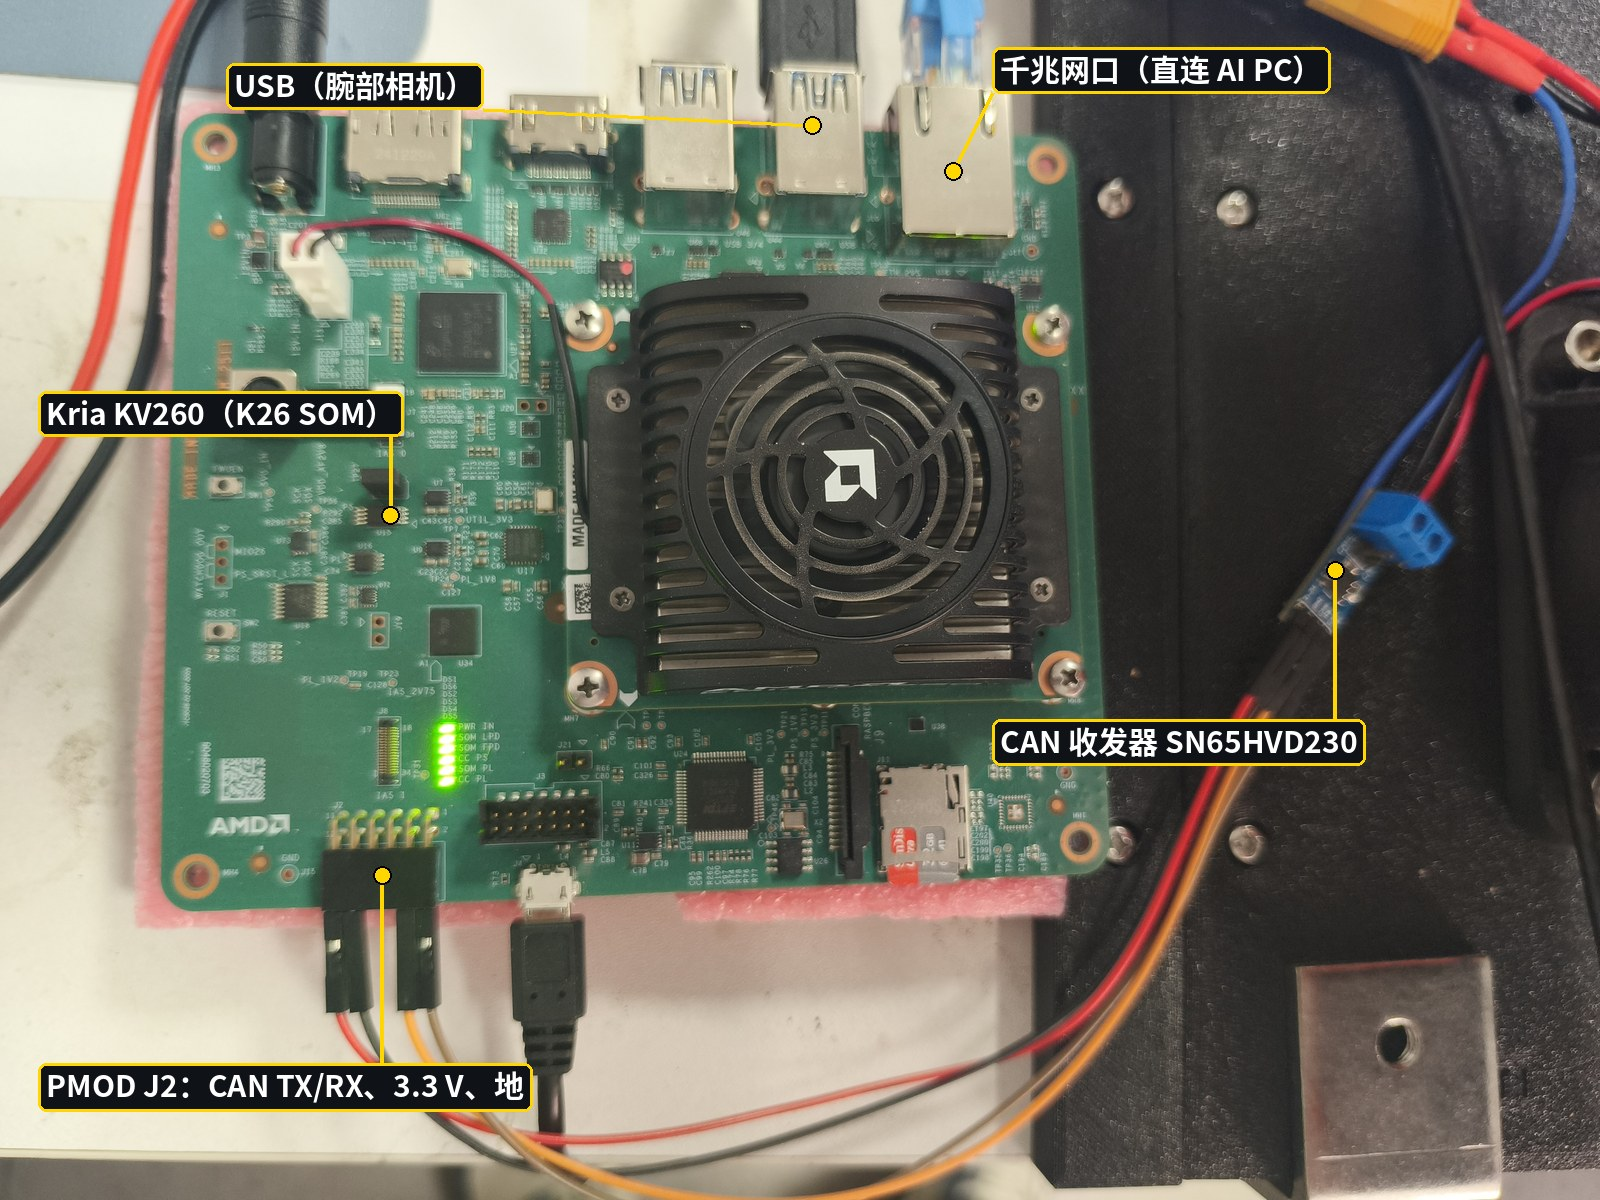
\includegraphics[width=.8\linewidth]{kv260_wiring.jpg}
  \caption{KV260 与 CAN 收发器接线}\label{fig:kv260}
\end{figure}

\subsubsection{软件成果}

上位机控制台集中显示中文指令、解析结果、执行进度、每件零件的对准用时和最终核验结果（图~\ref{fig:console}）。示教区域提供零重力启停、姿态记录和轨迹录制，数字孪生按实测关节角更新。板端软件按内容摘要发布，已有版本可复用，启动时校验源文件摘要，使作业与运行版本对应。

\subsection{特性成果}

\subsubsection{零件识别精度与端侧推理}

四类实例分割模型 YOLO11n-seg 在 AI PC 上用 ROCm 训练，验证集掩码 mAP50 为 0.976、mAP50-95 为 0.729，框 mAP50-95 为 0.852。量化后，用 80 帧图像对照 NPU 与 GPU 后端的抓取目标输出：匹配 270 个三维目标，可抓判定 270/270 一致，两后端输出的基座坐标差值 P50 为 0.33\,mm。\doccite{ref:yolo}

检测延迟见表~\ref{tab:det}。相机采集 1920×1080 图像，经缩放、填充后形成 736×1280 网络输入。后处理还原全分辨率掩码；验证使用 imgsz=1280。

\begin{table}[H]
\centering\small
\caption{头部检测单帧延迟（batch=1，1920×1080 原图，含全分辨率掩码，100 次）}\label{tab:det}
\begin{tabularx}{\linewidth}{@{}l C C C C@{}}
\toprule
后端 & 预处理 P50 & 推理 P50 & 后处理 P50 & 总延迟 P50 / P95 \\
\midrule
GPU（ROCm，FP32） & 8.7\ms & 29.8\ms & 4.6\ms & 45.4 / 49.1\ms \\
NPU（Quark A8W8） & 16.9\ms & 51.9\ms & 2.5\ms & 72.1 / 109.4\ms \\
\bottomrule
\end{tabularx}
\end{table}

\subsubsection{NPU/GPU 异构同载}

单独运行检测时，GPU 延迟较低；与大模型同时运行后，GPU 检测 P95 由 67\ms 升至 306\ms，NPU 检测 P95 由 120\ms 增至 141\ms（图~\ref{fig:contention}）。因此，系统将需要持续运行的分割任务部署到 NPU，把 GPU 留给大模型，以减轻并发推理对检测尾延迟的影响。

\begin{figure}[H]
  \centering
  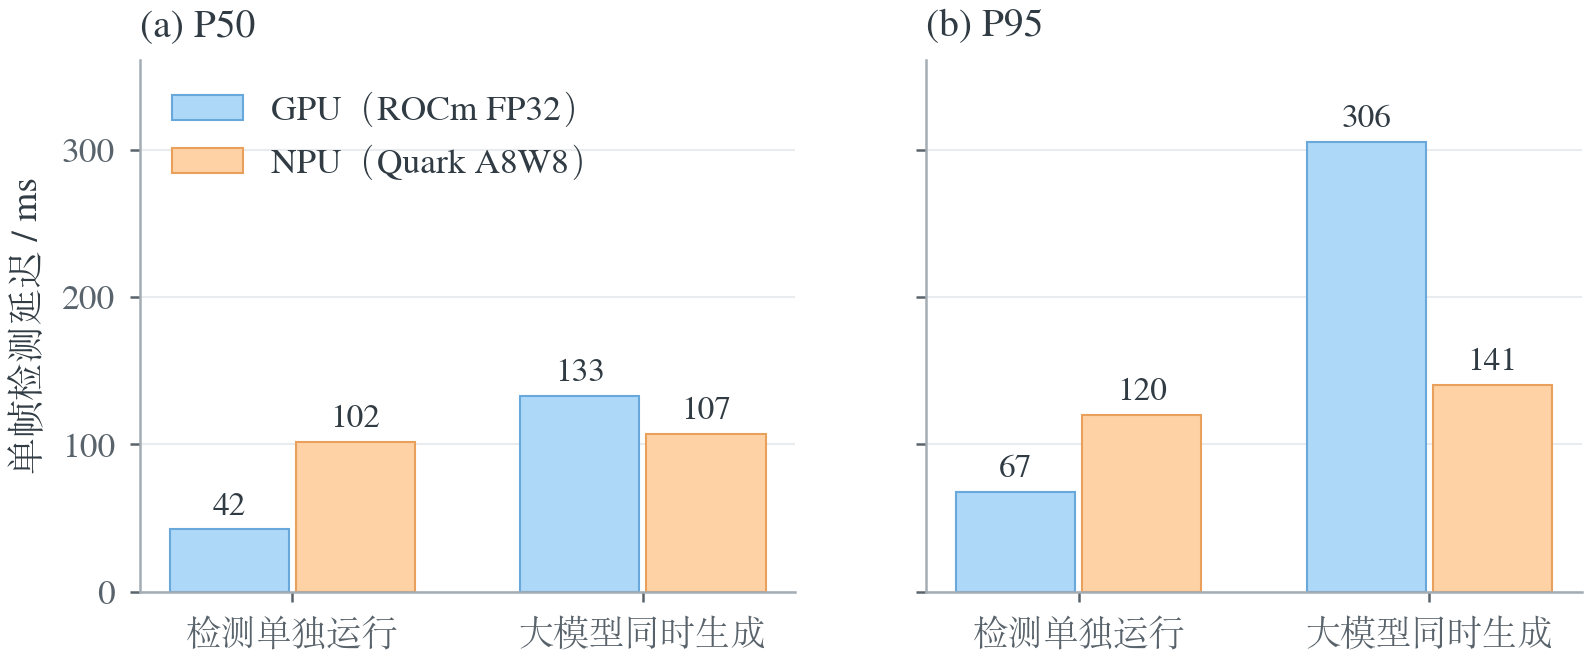
\includegraphics[width=\linewidth]{doc_contention.png}
  \caption{检测单独运行与大模型同时生成时的单帧检测延迟（每档 60 次）}\label{fig:contention}
\end{figure}

\subsubsection{5 ms 控制周期的线上实测}

用 Kingst LA2016 逻辑分析仪（50\,MHz 采样）在 CAN-H 上直接测量：位宽 1.0\us（1\,Mbps），总线占用 26.8\%。PL 轨迹流稳态段 77\,s、15364 个周期中，指令帧起点间隔 P50 4.9998\ms，周期间隔偏差 P50 0.4\us、P95 67.0\us。偏差按相邻指令帧起点间隔与 5\ms 的绝对差计算；周期锚定绝对时间栅格，图中晚点后的周期恢复到栅格，避免逐周期累积。游标实测相邻两个周期的同一指令帧起点相隔 4.99974\ms（图~\ref{fig:la}）。

\begin{figure}[H]
  \centering
  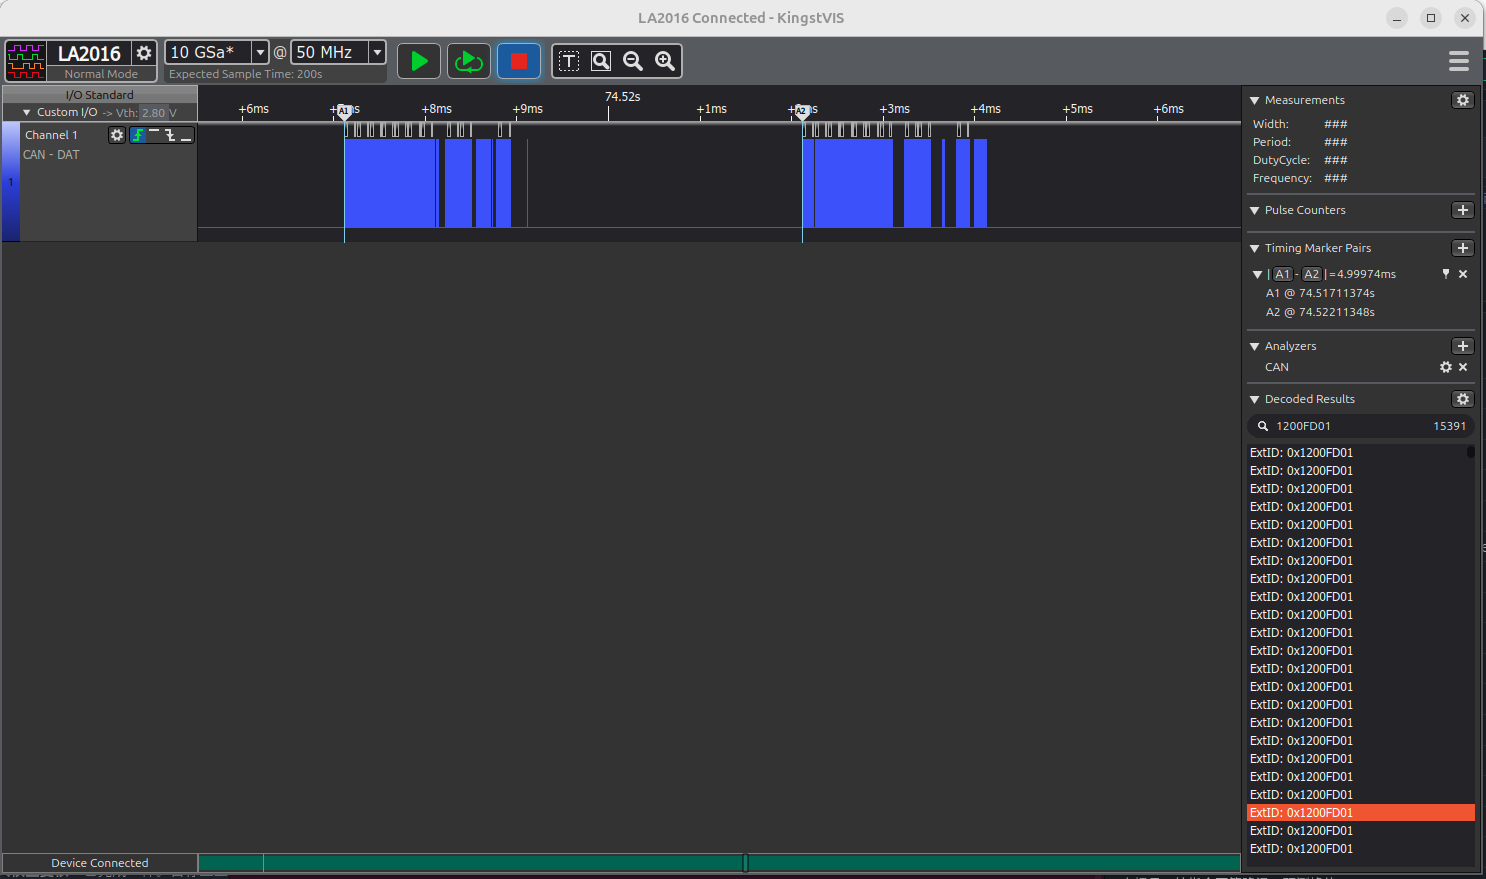
\includegraphics[width=.92\linewidth]{la_marker_5ms.png}
  \caption{逻辑分析仪实测：相邻两个 5 ms 周期的指令帧起点}\label{fig:la}
\end{figure}

\begin{figure}[H]
  \centering
  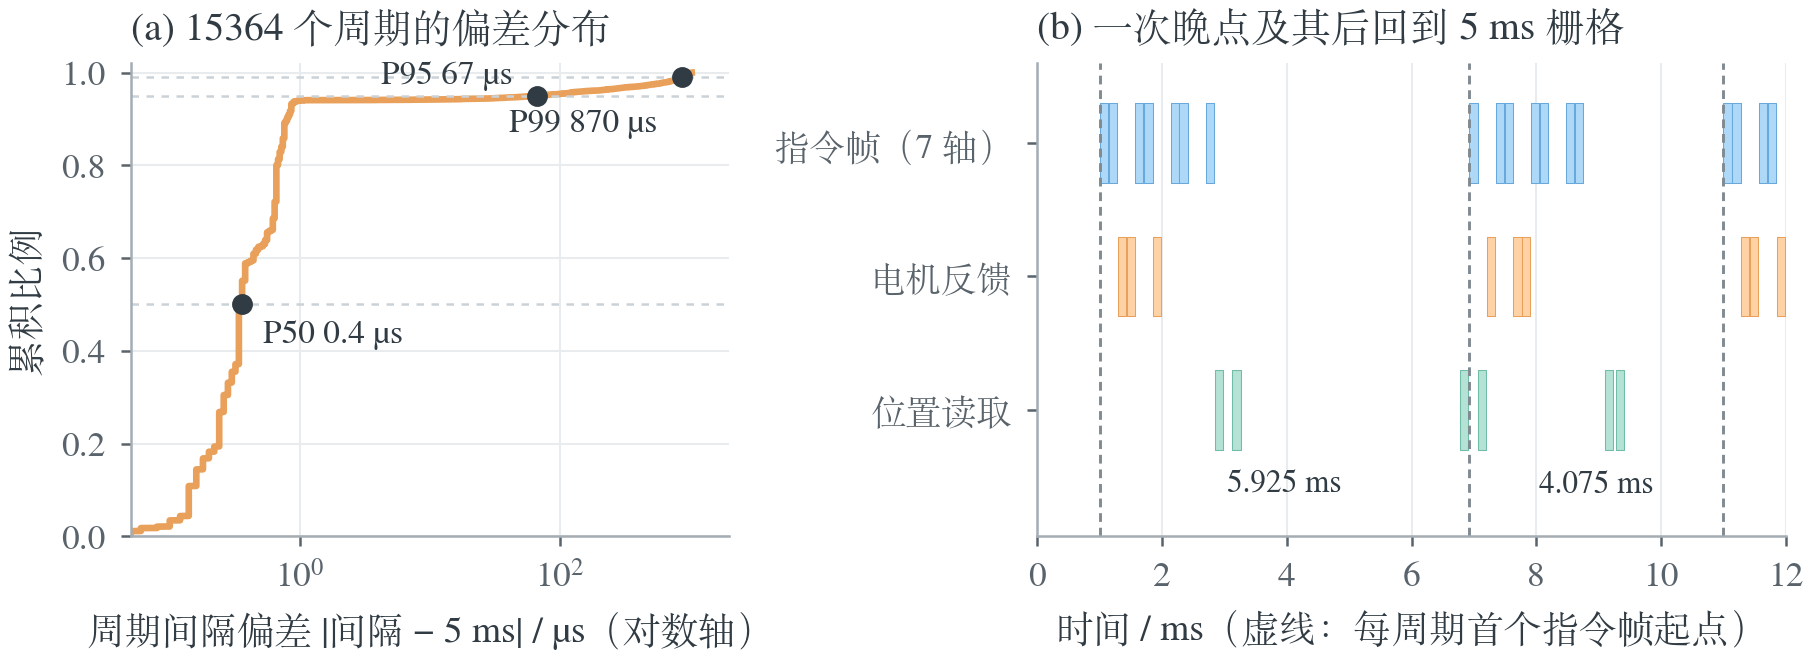
\includegraphics[width=\linewidth]{doc_wire.png}
  \caption{逻辑分析仪实测的 5 ms 周期：(a) 周期间隔偏差的累积分布；(b) 线上帧时序，晚点后下一周期回到栅格}\label{fig:wire}
\end{figure}

\subsubsection{关节跟踪与反馈时序}

一次完整四件运行（132\,s）中，J2 指令对反馈位置跟踪 RMSE 3.4\,mrad，J3 为 5.3\,mrad；七台电机反馈帧间隔（PL 1\us 计数器时间戳，名义 5\ms）P50 5.0\ms、P95 5.047\ms，间隔超过两倍中位数的次数为 0（图~\ref{fig:track}）。

\begin{figure}[H]
  \centering
  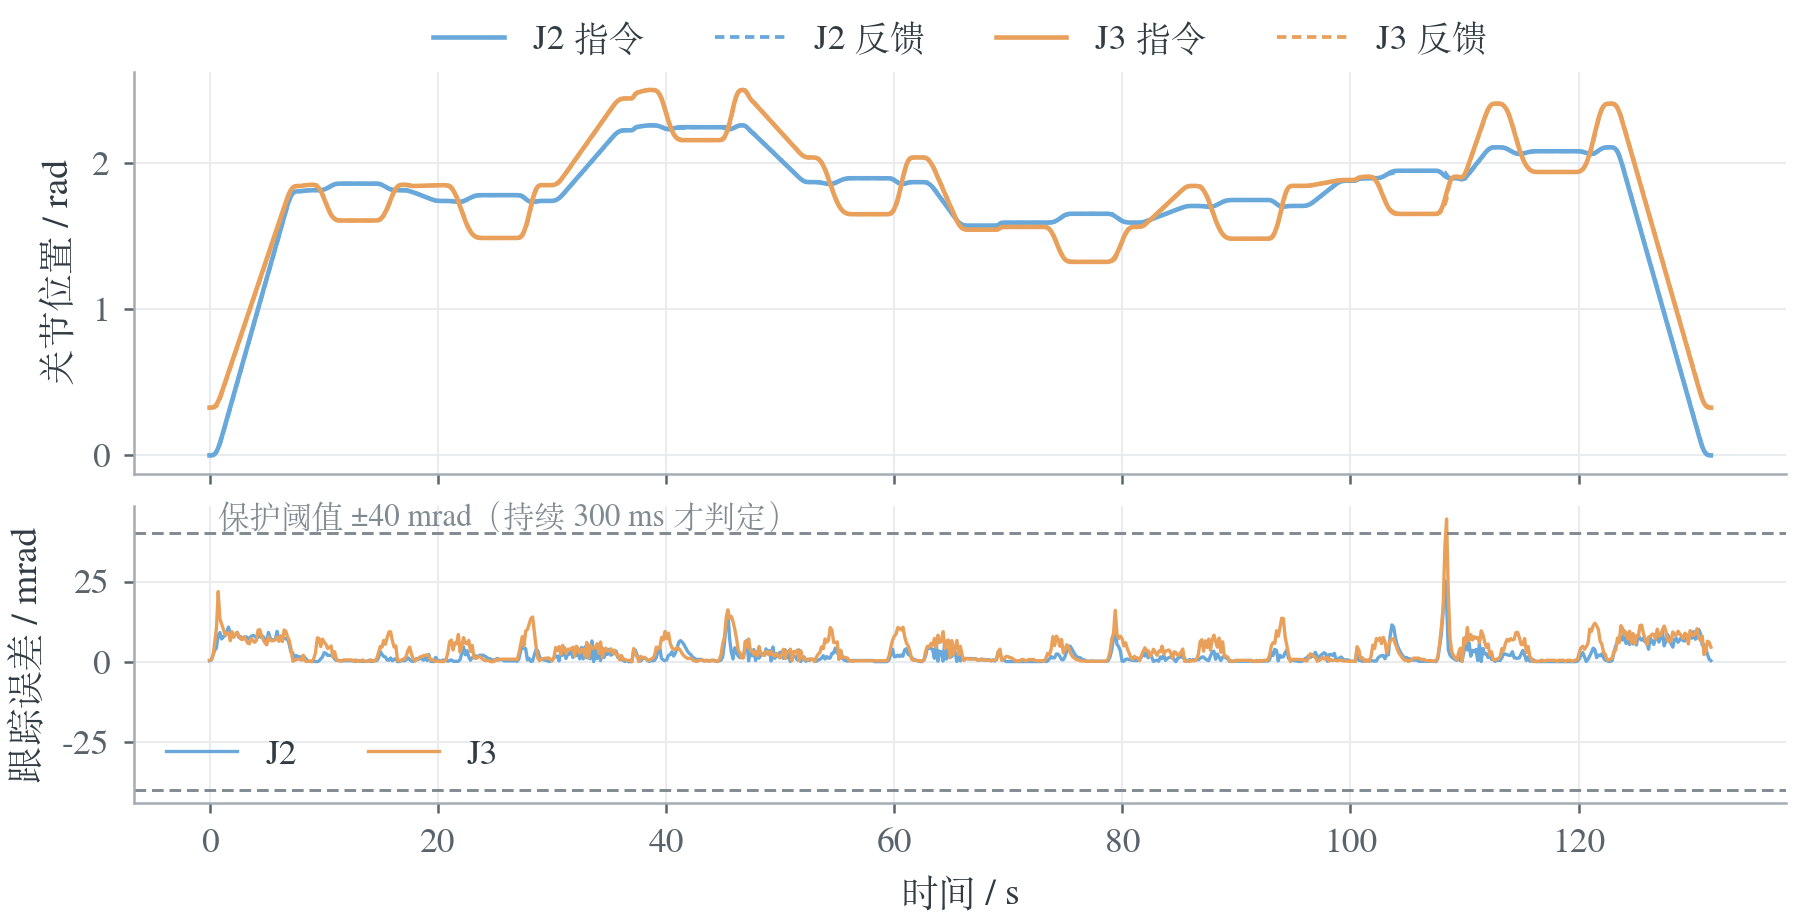
\includegraphics[width=\linewidth]{doc_tracking.png}
  \caption{一次完整四件运行中 J2、J3 的指令与反馈位置（上）及跟踪误差（下）}\label{fig:track}
\end{figure}

\subsubsection{板端闭环对准}

连续对准时，腕部定位与修正计算在 KV260 内完成。407 帧日志中，从腕部帧到达板端到写入 PL 修正目标的延迟 P50 为 123.0\ms、P95 为 206.0\ms，视觉环周期 P50 为 120.0\ms。从悬停到对准收敛，大螺丝用时 P50 为 1.06\,s（12/12 次收敛），大螺母为 2.43\,s（10/11 次收敛），小螺母为 1.61\,s（4/4 次收敛）。

图~\ref{fig:align} 同时列出历史停顿对准的 35 件记录，其悬停到开始下降用时 P50 为 6.67\,s；连续对准统计到收敛，两组计时终点分别标注。采用 CPU 核隔离后的 9 段记录中，各段控制心跳最大间隔的 P50 为 44.5\ms，全部记录的最大间隔为 51.7\ms，低于 PL 的 100\ms 租约。

\begin{figure}[H]
  \centering
  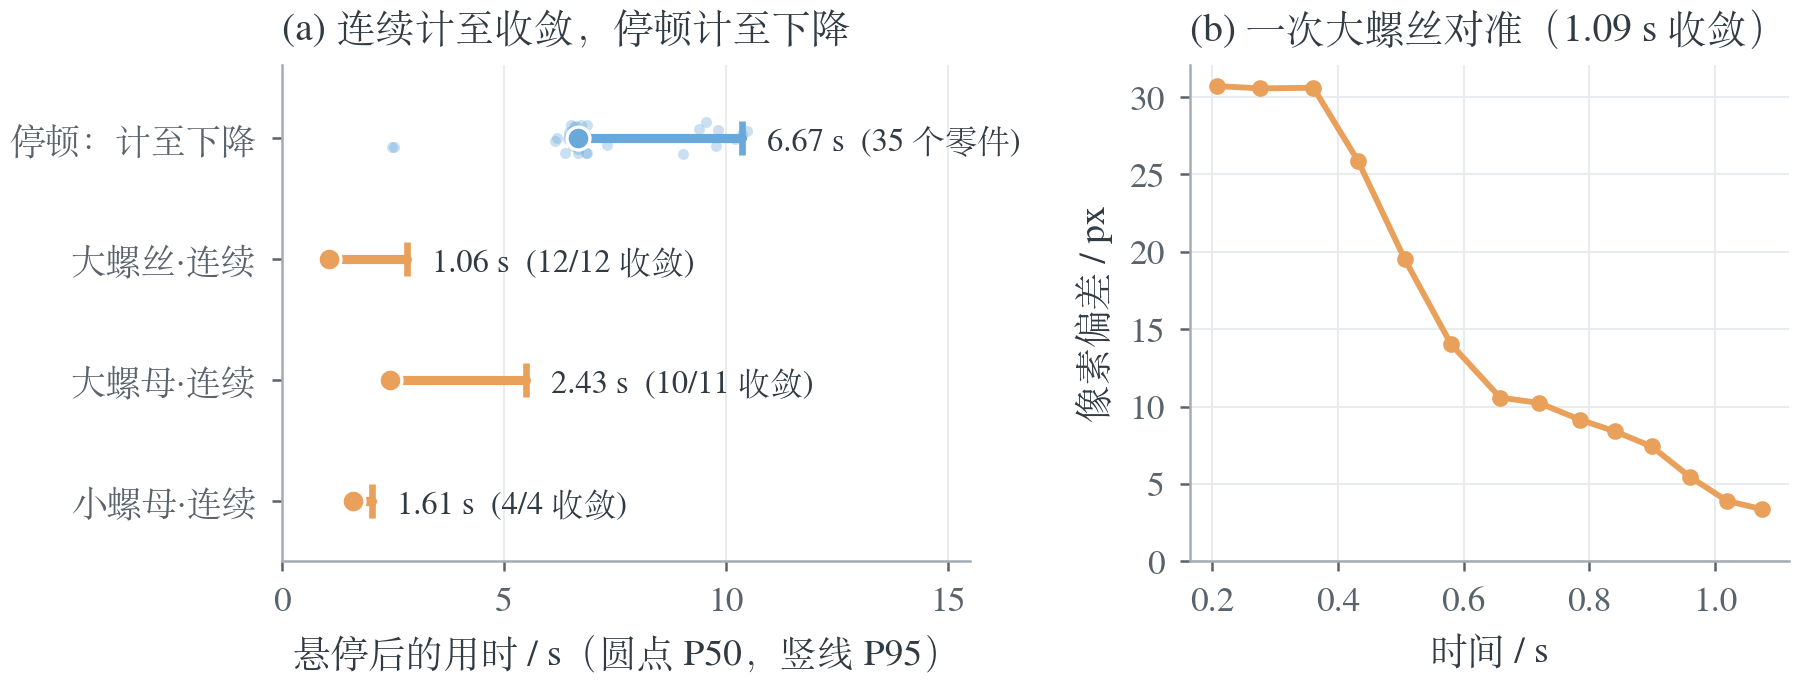
\includegraphics[width=\linewidth]{doc_alignment.png}
  \caption{(a) 连续对准计至收敛，停顿对准计至开始下降（浅色点为逐件数据）；(b) 一次大螺丝对准的像素偏差收敛过程}\label{fig:align}
\end{figure}

\subsubsection{PL 硬件加速与守护}

\begin{figure}[H]
  \centering
  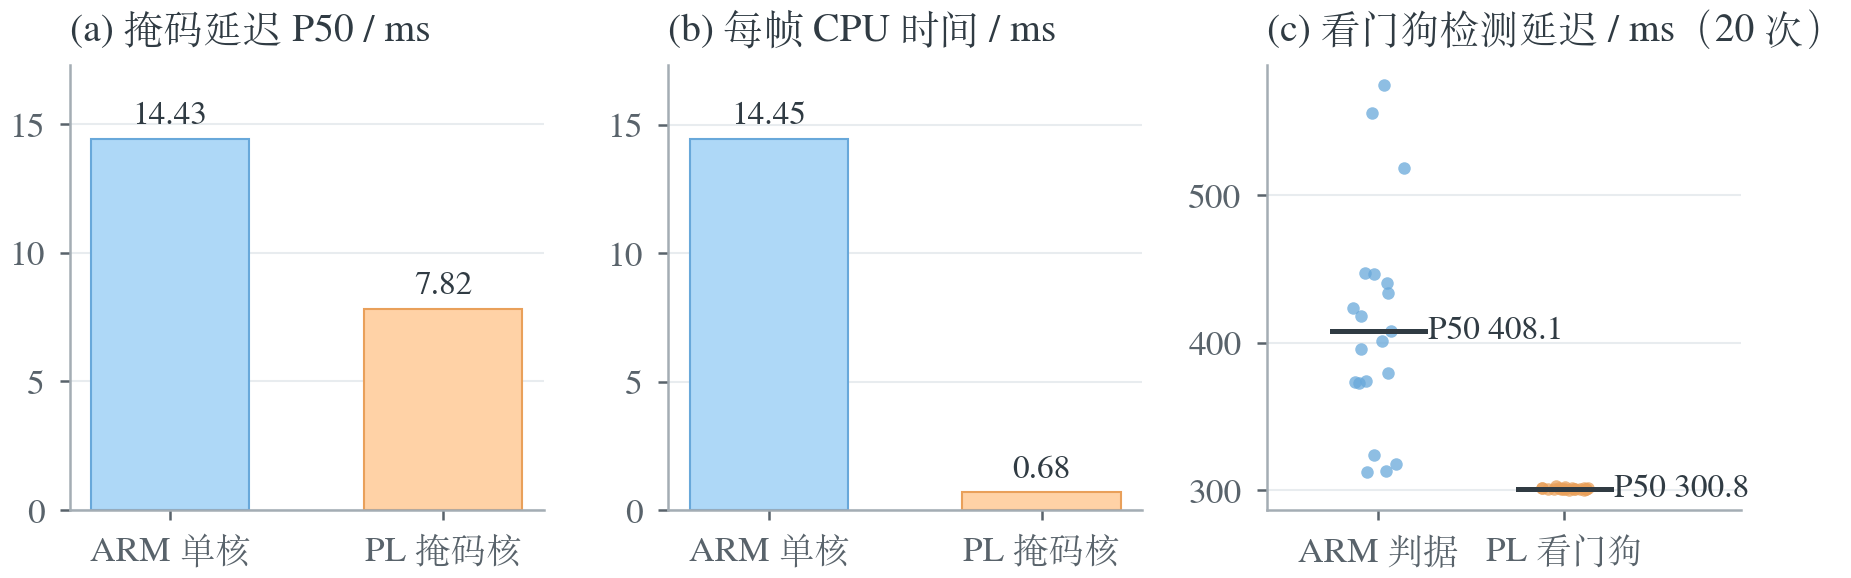
\includegraphics[width=\linewidth]{doc_pl_vs_arm.png}
  \caption{PL 与 ARM 实现对比：(a)(b) 腕部图像掩码，300 帧；(c) 七轴跟踪看门狗，逐次结果与中位数}\label{fig:plarm}
\end{figure}

\begin{table}[H]
\centering\small
\caption{PL 与 ARM 软件实现对比}\label{tab:plarm}
\begin{tabularx}{\linewidth}{@{}>{\raggedright\arraybackslash}p{3.4cm} c c Y@{}}
\toprule
功能 & PL & ARM & 说明 \\
\midrule
腕部图像掩码（P50） & 7.82\ms & 14.43\ms & 300 帧；每帧 CPU 耗时 0.68 对 14.45\ms，降低 95\%；结果逐位一致 \\
控制服务暂停 20\ms 时最长命令间隔 & 5.014\ms & 21.435\ms & 同一参考轨迹 ABBA 对照，PL 维持已提交轨迹的发送节拍 \\
跟踪看门狗检测延迟（P50） & 300.8\ms & 408.1\ms & 20 次板内回环测试；PL 逐帧判定七轴 \\
抓取轨迹 MMIO 写入次数 & \multicolumn{2}{c}{降低 87.59\%} & PL 段提交替代 ARM 逐拍写 \\
\bottomrule
\end{tabularx}
\end{table}

\subsubsection{通信与功耗}

AI PC 与 KV260 千兆直连，200 个 ICMP 包的 RTT P50 为 0.169\ms、P99 为 0.25\ms，测量期间零丢包。作业包通道的有效吞吐为 AI PC 到 KV260 28.2\,MB/s、反向 32.3\,MB/s。

AI PC 的 SoC 功率在空闲、GPU 检测循环和 NPU 检测循环下分别为 23.0\,W、55.6\,W 和 54.3\,W。KV260 测量的是整板功率，空闲为 3.34\,W，A53 单核执行掩码处理时为 3.68\,W。

\subsubsection{任务完成情况}

系统已完成四类零件从指令解析、目标识别到抓取放置、逐槽核对和中文复审的流程，并记录了四件零件在一次会话中全部完成搬运、核对通过的实例。任务接口支持按类别和数量分拣；大螺丝还完成了双向搬运与目标数量调节，可按“多的退回、少的补入”调整目标盘数量。示教与数字孪生提供姿态记录和状态观察。

2026-10-28 至 2026-11-01 的开发记录中，数量统计完整的任务共计划放置 104 件，头部相机确认 83 件，确认比例为 79.8\%。逐次任务、放置核对和运行数据保存在 \path{metrics/logs/task_trials.csv}，典型完整运行的跟踪与对准数据见本节图表。